\chapter{Functionality}

The Setlx-addition SetlCup is a LR-Parser-Generator based on JavaCup.
The idea is to use a user given scanner- and parser-definition and create an AST out of a given input using the definitions.

In this document the needed syntax of the definitions is examined and the given output is evaluated.

A sample input file is divided into three Sections:
\begin{enumerate}
	\item Commentpart
	\item Scanner-Part
	\item Parser-Part
\end{enumerate}

At first the correct call of the program is discussed.
\section{Using SetlCup}
SetlCup has multiple different variants in which it can be called:
\subsection{Calling via comment prompt}
\begin{enumerate}
	\item \begin{Verbatim}
	setlx setlcup.stlx -p parser_scanner_file.stlx file_to_be_read.txt 
	\end{Verbatim}
			With this call there will be no output for the user.
	\item \begin{Verbatim}
	setlx setlcup.stlx -p parser_scanner_file.stlx file_to_be_read.txt -d
	\end{Verbatim}
			With this call debugging is possible. It shows the different tables and states and the whole parsing progress. HINT: It is recommended to pipe the output into a file if you are using the "-d" option.
	\item \begin{Verbatim}
	setlx setlcup.stlx -h
	\end{Verbatim}
			With this call a little help will be showed, on how to call SetlCup correctly.
\end{enumerate}
\subsection{Calling via Setlx}
SetlCup can also be called in Setlx itself. If this case is used, you need to load the program "setlcup\_load.stlx".
%\begin{figure}[!ht]
%\begin{Verbatim}[ frame         = lines, 
                  %framesep      = 0.3cm, 
                  %labelposition = bottomline,
                  %numbers       = left,
                  %numbersep     = -0.2cm,
                  %xleftmargin   = 0.8cm,
                  %xrightmargin  = 0.8cm,
                %]
	%load("setlcup_load.stlx");
%\end{Verbatim}
%\end{figure}
Afterwards Setlcup can be used via the method call
\begin{Verbatim}
	call_generate_ast(input_grammar, file_to_parse, silent_mode);
\end{Verbatim}

e.g.
\begin{figure}[!ht]
\begin{Verbatim}[ frame         = lines, 
                  framesep      = 0.3cm, 
                  labelposition = bottomline,
                  numbers       = left,
                  numbersep     = -0.2cm,
                  xleftmargin   = 0.8cm,
                  xrightmargin  = 0.8cm,
                ]
	load("setlcup_load.stlx");
	print(call_generate_ast('examples\math_expression_grammar_ast.g', 
	                    'examples\math_expression_input.txt', true));
\end{Verbatim}
\end{figure}
\section{Comment-Part}
In the comment-part everything which is written will not be used by the Program itself. It is adviced to comment your idea behind the parser and scanner structure in this section.
The section is ended with the "\%\%\%" symbol.

\section{Scanner-Part}
The scanner is responsible for checking whether the input file consists of the defined tokens. It can be written like this:
\begin{figure}[!ht]
\begin{Verbatim}[ frame         = lines, 
                  framesep      = 0.3cm, 
                  labelposition = bottomline,
                  numbers       = left,
                  numbersep     = -0.2cm,
                  xleftmargin   = 0.8cm,
                  xrightmargin  = 0.8cm,
                ]
	INTEGER       := 0|[1-9][0-9]*     ;
	ASTERISK      := \*                ;
	WHITESPACE    := [ \t\v\r\s]       ;
	SKIP          := {WHITESPACE} | \n ;
\end{Verbatim}
\caption{Scanner Definition}
\label{fig:scanner_def}
\end{figure}
\begin{itemize}
	\item In line 1 the Token "INTEGER" is defined. Tokens are defined in the following way:\\
					token\_name := regex ;
	\item In line 2 it is shown, that predefined tokens in Regular Expressions like "$*,+,?,|,\{,\},(,),\cdots$" need to be escaped.
	\item In line 3 the "Whitespace" symbols are demonstrated.
	\item In Line 4 the "SKIP"-Token is shown. In some contexts tokens like Whitespaces are not needed. They can be skipped by defining the "SKIP"-Token with "\{TOKENNAME\}" of the respective tokens, which shall be skipped. Multiple tokens need to be seperated by a pipe "|". It is also possible to skip by inserting a regex itself.
\end{itemize}

\section{Parser-Part}
In this part the grammar-rules are defined with the following syntax:
\begin{figure}[!ht]
\begin{Verbatim}[ frame         = lines, 
                  framesep      = 0.3cm, 
                  labelposition = bottomline,
                  numbers       = left,
                  numbersep     = -0.2cm,
                  xleftmargin   = 0.8cm,
                  xrightmargin  = 0.8cm,
                ]
	expr ::= 
	  expr:e MINUS prod:p {: result := Minus(e,p);:} 
	| expr:e '+' prod:p   {: result := Plus(e,p); :} 
	| 										{: :}
	;
\end{Verbatim}
\caption{Example grammar rule}
\label{fig:example_grammer}
\end{figure}
\begin{itemize}
	\item[rule\_head] The rule\_head is the name of the rule i.e. "expr". It is possible to reference defined rules via their rule\_name
	\item[body\_list] The rule can consist of multiple bodys.
	\item[rule\_body] The body can contain multiple elements. 
	\item[rule\_element] A rule element is either a :
	\begin{enumerate}
		\item Token (defined in the scanner) e.g. "MINUS"
		\item Token in  ' ' e.g. '+' as a literal
		\item other rule\_heads e.g. "prod"
	\end{enumerate}
	The Tokens defined in the scanner, as well as the rule\_heads can have an id. This can be used in the action\_code.
	\item[action\_code] The action\_code is an optional part in a body. It needs to be at the end of the body it self. Each rule\_element can have an action\_code. In this action\_code Setlx Code can be written. By using the variable "result" it is possible to pass values between rules. The id of the elements in the respective rule can be referred to by using its name.
	\item[|] The pipe separates the different bodies.
\end{itemize}
\newpage
\section{Example}
The first example shows a simple arithmetic grammar.
The second example shows how a simple programming language can be parsed using SetlCup.
\subsection{Arithmetic grammar}
The arithmetic grammar and scanner is the following \ref{fig:example_arithmetic_grammer}.
\begin{figure}[!ht]
\begin{Verbatim}[ frame         = lines, 
                  framesep      = 0.3cm, 
                  labelposition = bottomline,
                  numbers       = left,
                  numbersep     = -0.2cm,
                  xleftmargin   = 0.8cm,
                  xrightmargin  = 0.8cm,
                ]
  %%%

  INTEGER       := 0|[1-9][0-9]* ;
  WHITESPACE    := [ \t\v\r\s] ;
  SKIP          := {WHITESPACE} | \n ;

  %%%
  arith_expr 
   ::= expr_list:esl                {: result := ExprList(esl); :};

  expr_list 
   ::= expr_part:part expr_list:l {: result := [part] + l; :} 
     |                            {: result := []; :}
     ;
  expr_part 
   ::= expr:e ';'            {: result := e; :} ;
  expr 
   ::=  expr:e '+'  prod:p   {: result := Plus(e , p);  :} 
     |  expr:e '-'  prod:p   {: result := Minus(e , p); :} 
     |  prod:p               {: result := p;     :}
     ;
  prod 
   ::=  prod:p '*'  fact:f   {: result := Times(p , f); :}
     |  prod:p DIVIDE fact:f {: result := Div(p , f); :} 
     |  prod:p '%'    fact:f {: result := Mod(p , f); :} 
     |  fact:f               {: result := f;     :}
     ;
  fact 
   ::=  '(' expr:e_part ')'   {: result :=  e_part ;   :} 
     |  INTEGER:n             {: result := Integer(eval(n)); :} 
     ;
\end{Verbatim}
\caption{Example arithmetic grammar}
\label{fig:example_arithmetic_grammer}
\end{figure}
%\lstinputlisting[frame=single,numbers=left,basicstyle=\footnotesize]{math_expression_grammar_ast.g}
A sample input file\ref{fig:example_arithmetic_input}.
\begin{figure}[!ht]
\begin{Verbatim}[ frame         = lines, 
                  framesep      = 0.3cm, 
                  labelposition = bottomline,
                  numbers       = left,
                  numbersep     = -0.2cm,
                  xleftmargin   = 0.8cm,
                  xrightmargin  = 0.8cm,
                ]
  1 + 2 * 3 - 4;
  1 + 2 + 3 + 4;
  1 + ( 2 * 3 ) * 5 % 6;
\end{Verbatim}
\caption{Example arithmetic input}
\label{fig:example_arithmetic_input}
\end{figure}
%\lstinputlisting[frame=single,numbers=left,basicstyle=\footnotesize]{math_expression_input.txt}
The output AST:
%\lstinputlisting[basicstyle=\footnotesize,breaklines=true]{math_expression_output.txt}

\begin{figure}[!ht]
	\centering
		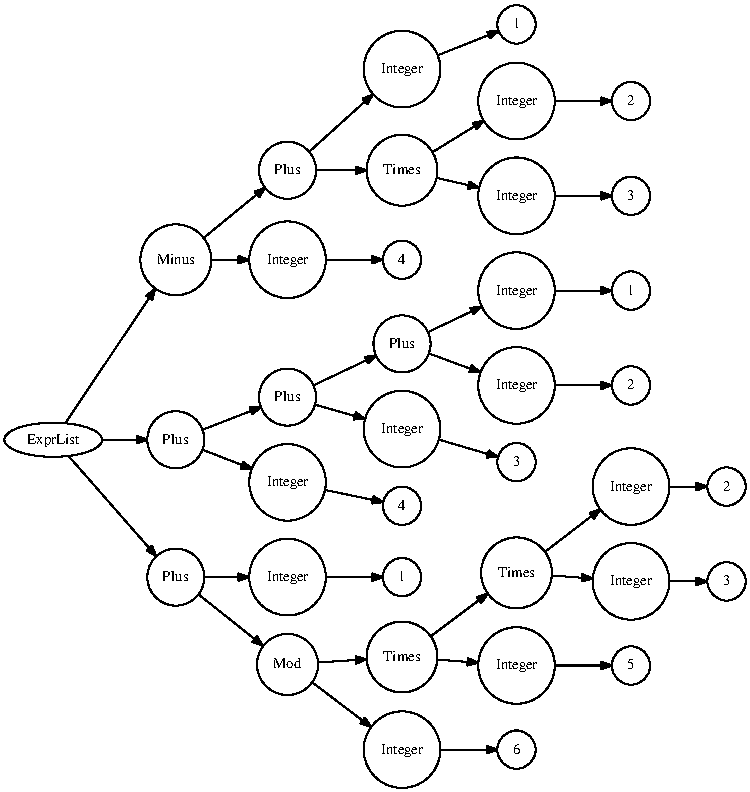
\includegraphics{arith_expr_tree.pdf}
	\caption{Arithexpr AST}
	\label{fig:arith_expr_tree}
\end{figure}

\subsection{Programming language grammar}
The programming language grammar and scanner.
The Scanner \ref{fig:example_interpreter_grammar_scanner}.
The Statements \ref{fig:example_interpreter_grammar_statements}.
The Lists \ref{fig:example_interpreter_grammar_lists}.
The Expressions \ref{fig:example_interpreter_grammar_expression}.
%\lstinputlisting[frame=single,numbers=left,basicstyle=\footnotesize ,breaklines=true]{interpreter_grammar_ast.g}
\begin{figure}[!ht]

\begin{Verbatim}[ frame         = lines, 
                  framesep      = 0.3cm, 
                  labelposition = bottomline,
                  numbers       = left,
                  numbersep     = -0.2cm,
                  xleftmargin   = 0.8cm,
                  xrightmargin  = 0.8cm,
                ]
  %%%
  FUNCTION    := function ;
  RETURN      := return ;
  IF          := if ;
  ELSE        := else ;
  WHILE       := while ;
  FOR         := for ;
  PRINT       := print ;
  QUIT        := exit ;
  STRING      := \"(?:\\.|[^\"])*\" ;
  WHITESPACE  := [ \t\v\r\s] ;
  SKIP        := {WHITESPACE}|\n|//[^\n]* ;
  INTEGER     := 0|[1-9][0-9]* ;
  DECIMAL     := 0\.[0-9]+|[1-9][0-9]*\.[0-9]+ ;
  ZID         := [a-zA-Z_][a-zA-Z0-9_]* ;  
  %%%
\end{Verbatim}
\caption{Example interpreter scanner}
\label{fig:example_interpreter_grammar_scanner}
\end{figure}
\begin{figure}[!ht]

\begin{Verbatim}[ frame         = lines, 
                  framesep      = 0.3cm, 
                  labelposition = bottomline,
                  numbers       = left,
                  numbersep     = -0.2cm,
                  xleftmargin   = 0.8cm,
                  xrightmargin  = 0.8cm,
                ]
  program 
   ::= dfnStmntList:d {: result := Program(d); :}
     ;
  dfnStmntList 
   ::= definition:d dfnStmntList:dl       {: result := [d] + dl; :}
     |  statement:stmts  dfnStmntList:dsl {: result := [stmts] + dsl; :}
     |                                    {: result := []; :}
     ;
  definition 
   ::= FUNCTION ZID:function_name '(' paramList:param_list ')' 
			'{' stmntList:statement_list '}'
       {: result := Function(function_name, param_list, statement_list);:}
     ;
  stmntList
   ::= statement:s stmntList:sl {: result := [s] + sl ; :}
     |  {: result := []; :}
     ;
  statement 
   ::= assignment:a ';'   {: result := Assign(a); :}    
     |  PRINT '(' printExprList:printexpr_list ')' ';'      
                          {: result := Print(printexpr_list); :}
     |  IF '(' boolExpr:b ')' '{' stmntList:st_list1 '}'    
                          {: result := If(b, st_list1); :}
     |  WHILE '(' boolExpr:b ')' '{' stmntList:st_list2 '}' 
                          {: result := While(b, st_list2); :}
     |  FOR '(' assignment:i_a ';' boolExpr:b ';' assignment:e_a ')' 
		    '{' stmntList:st_list3 '}' 
                          {: result := For(i_a, b, e_a, st_list3);  :}
     |  RETURN expr:e ';' {: result := Return(e); :}
     |  RETURN ';'        {: result := Return();  :}
     |  expr:e ';'        {: result := Expr(e);   :}      
     |  QUIT ';'          {: result := Exit();    :}
     ;
\end{Verbatim}
\caption{Example interpreter statements}
\label{fig:example_interpreter_grammar_statements}
\end{figure}
\begin{figure}[!ht]

\begin{Verbatim}[ frame         = lines, 
                  framesep      = 0.3cm, 
                  labelposition = bottomline,
                  numbers       = left,
                  numbersep     = -0.2cm,
                  xleftmargin   = 0.8cm,
                  xrightmargin  = 0.8cm,
                ]
  printExprList 
   ::= printExpr:p ',' nePrintExprList:np {: result := [p] + np ; :}
     |  printExpr:p                       {: result := [p]; :}
     |                                    {: result := [];  :}
     ;
  nePrintExprList
   ::= printExpr:p                         {: result := [p]; :}
     |  printExpr:p ',' nePrintExprList:np {: result := [p] + np ; :}
     ;
  printExpr 
   ::= STRING:string {: result := PrintString(string); :}
     |  expr:e       {: result := e; :}
     ;
  assignment 
   ::= ZID:id '=' expr:e {: result := Assign(id, e); :}
     ;
  paramList 
   ::= ZID:id ',' neIDList:nid {: result := [id] + nid ; :}
     |  ZID:id                 {: result := [id] ; :}
     |                         {: result := []; :}
     ;
  neIDList
   ::= ZID:id ',' neIDList:nid {: result := [id] + nid ; :}
     |  ZID:id                 {: result := [id] ; :}
     ;
  exprList
   ::= expr:e ',' neExprList:el {: result := [e] + el; :}
     |  expr:e                  {: result := [e]; :}
     |                          {: result := [];  :}
     ;
  neExprList
   ::= expr:e ',' neExprList:el {: result := [e] + el; :}
     |  expr:e                  {: result := [e]; :}
     ;
		\end{Verbatim}
\caption{Example interpreter Lists}
\label{fig:example_interpreter_grammar_lists}
\end{figure}
\begin{figure}[!ht]

\begin{Verbatim}[ frame         = lines, 
                  framesep      = 0.3cm, 
                  labelposition = bottomline,
                  numbers       = left,
                  numbersep     = -0.2cm,
                  xleftmargin   = 0.8cm,
                  xrightmargin  = 0.8cm,
                ]
  boolExpr 
   ::= expr:lhs '==' expr:rhs                {: result := Equation(lhs,rhs); :}
     |  expr:lhs '!=' expr:rhs               {: result := Inequation(lhs,rhs); :}
     |  disjunction:lhs '==' disjunction:rhs {: result := Equation(lhs,rhs); :}
     |  disjunction:lhs '!=' disjunction:rhs {: result := Inequation(lhs,rhs); :}
     |  expr:lhs '<=' expr:rhs               {: result := LessOrEqual(lhs,rhs);    :}
     |  expr:lhs '>=' expr:rhs               {: result := GreaterOrEqual(lhs,rhs); :}
     |  expr:lhs '<' expr:rhs                {: result := LessThan(lhs,rhs); :}
     |  expr:lhs '>' expr:rhs                {: result := GreaterThan(lhs,rhs); :}
     |  disjunction:d                        {: result := d; :}
     ;
  disjunction
   ::= disjunction:d '||' conjunction:c {: result := Disjunction(d,c); :}
     |  conjunction:c                   {: result := c; :}
     ;
  conjunction
   ::= conjunction:c '&&' boolFactor:f {:result := Conjunction(c,f); :}
     | boolFactor:f                    {: result := f; :}
     ;
  boolFactor
   ::= '(' boolExpr:be_par ')' {:  result := be_par; :}
     | '!' boolExpr:e          {: result := Negation(e); :}
     ;
  expr 
   ::= expr:e '+'   prod:p {: result := Sum(e,p); :} 
     |  expr:e '-'  prod:p {: result := Difference(e,p); :} 
     |  prod:p             {: result := p;     :}
     ;
  prod 
   ::= prod:p '*'  fact:f    {: result := Product(p,f); :}
     |  prod:p '\' fact:f    {: result := Quotient(p,f); :} 
     |  prod:p '%' fact:f    {: result := Mod(p,f); :} 
     |  fact:f               {: result := f;     :}
     ;
  fact 
   ::= '(' expr:e_par ')'            {: result := e_par;   :} 
     |  INTEGER:n                    {: result := Integer(eval(n));   :} 
     |  DECIMAL:d                    {: result := Decimal(eval(d)); :}
     |  ZID:id_1 '(' exprList:el ')' {: result := FunctionCall(id_1,el); :}
     |  ZID:id_2                     {: result := Variable(id_2); :}
     ;
		\end{Verbatim}
\caption{Example interpreter expressions}
\label{fig:example_interpreter_grammar_expression}
\end{figure}
A sample input file \ref{fig:example_interpreter_input}.
\begin{figure}[!ht]

\begin{Verbatim}[ frame         = lines, 
                  framesep      = 0.3cm, 
                  labelposition = bottomline,
                  numbers       = left,
                  numbersep     = -0.2cm,
                  xleftmargin   = 0.8cm,
                  xrightmargin  = 0.8cm,
                ]
  function factorial(n) {
      if (n == 0) {
         return 1;
      }
      return n * factorial(n - 1);
  }
  print("Calculation of factorial for i = 1 to 9");
  for (i = 0; i < 10; i = i + 1) {
      print(i, "! = ", factorial(i));
  }
  print();
		\end{Verbatim}
\caption{Example interpreter input}
\label{fig:example_interpreter_input}
\end{figure}
%\lstinputlisting[frame=single,numbers=left,basicstyle=\footnotesize ,breaklines=true]{factorial.sl}
The output AST:
%\lstinputlisting[basicstyle=\footnotesize ,breaklines=true]{factorial_output.txt}


\begin{figure}
	\centering
		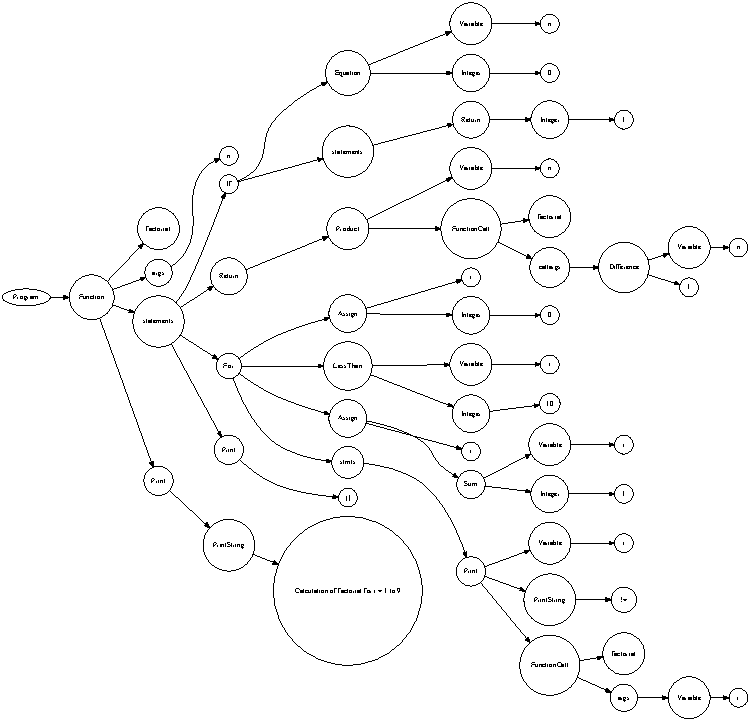
\includegraphics{interpreter_tree.pdf}
	\caption{Interpreter AST}
	\label{fig:interpreter_tree}
\end{figure}

